\documentclass{extbook}
\usepackage[papersize={8.5in,11in},top=1in,bottom=1in]{geometry}
\RequirePackage{fix-cm}
\usepackage[T1]{fontenc}
\usepackage{lmodern}
\usepackage{fullpage}
\usepackage{titlesec}
\usepackage{parskip}
\usepackage{float}
\usepackage{url}
\usepackage{hyperref}
\usepackage{graphicx}
\usepackage{tcolorbox}
\usepackage{tabularx}
\usepackage{xcolor}
\usepackage{titlesec}
\usepackage{amsmath}
\usepackage{listings}
\usepackage{tcolorbox}
\usepackage{tabularx}


\lstset
{
    breaklines=true,
    tabsize=3,
    showstringspaces=false
}

\lstdefinestyle{vbstyle}{
  language={[Visual]Basic},
  backgroundcolor=\color{lightgray}, % Color de fondo
  basicstyle=\ttfamily\small, % Tamanoo y tipo de fuente
  keywordstyle=\color{blue}, % Color para palabras clave
  commentstyle=\color{green}, % Color para comentarios
  stringstyle=\color{red}, % Ccadenas de texto
  numberstyle=\tiny\color{gray}, % Coñor y tamaño de los números de línea
  stepnumber=1,
  numbers=left, % esto es para el # de la linea
  numbersep=5pt,
  showstringspaces=false,
  frame=single,
  breaklines=true
}

\renewcommand{\contentsname}{Contenido}
\renewcommand{\figurename}{Figura}
\renewcommand{\listtablename}{Lista de tablas}
\renewcommand{\listfigurename}{Lista de figuras}
\usepackage[fontsize=13.5pt]{fontsize}
\setlength{\parindent}{0pt}

\titleformat{\chapter}[display]
  {\bfseries\huge} % Estilo del título
  {\hfill\Large} % Alineación a la derecha
  {3ex} % Espaciado entre el número del capítulo y el título
  {\vspace{-5cm}\titlerule\vspace{1.5ex}\hfill} % Regla arriba y alineación del título a la derecha
  [\vspace{1ex}\titlerule] % Regla debajo del título


  \makeatletter
  \patchcmd{\chapter}
    {\if@openright\cleardoublepage\else\clearpage\fi}
    {\clearpage}
    {}{}
  \makeatother

  \definecolor{codegreen}{rgb}{0,0.6,0}
  \definecolor{codegray}{rgb}{0.5,0.5,0.5}
  \definecolor{codepurple}{rgb}{0.58,0,0.82}
  \definecolor{backcolour}{rgb}{0.95,0.95,0.92}

\begin{document}
\begin{titlepage}
  \begin{center}
      {\huge \textbf{Universidad Tecnológica de Panamá}}\\
      \vspace{3mm}
      {\Large \textbf{Centro Regional De Veraguas}}

      \begin{figure}[H]
          \centering
          
\includegraphics[scale = 0.07]{Imagenes/utp.png}
          
\includegraphics[scale = 0.58]{Imagenes/fisc.png}
      \end{figure}
      {\Large \textbf{Facultad de Ingeniería de Sistemas Computacionales}}\\
      \vspace{5mm}
      
      {\Large \textbf{Curso: Herramientas de Programación Aplicada III}}\medskip
      
      {\Large \textbf{Profesora: Milka de Escobar}}

      \rule{\linewidth}{0.75mm}\\
          {\Large \textsc{Informe de asignación 2}} 
      \rule{\linewidth}{0.75mm}\medskip

      {\Large \textbf{Estudiantes}}\\
      \vspace{5mm}
      {\Large \textbf{Elbin Puga, Arland Barrera}}
      \vfill
      {\Huge \textbf{2024}}

  \end{center}
\end{titlepage}
\tableofcontents
\listoffigures
%\listoftables para lista de tablas 
\chapter{Introducción}
En esta asignación se desarrolló un programa que calcula el área y el perímetro de dos figuras geométricas: el trapecio y el triángulo. El objetivo principal fue aplicar los conocimientos adquiridos en el curso de Herramientas de Programación Aplicada III, utilizando herramientas básicas de interfaz gráfica como Textbox para la entrada de datos y Label para mostrar los resultados. Este tipo de aplicación refuerza conceptos de geometría, así como habilidades de programación orientada a objetos y diseño de interfaces de usuario.

El programa fue diseñado para ser lo suficientemente flexible y fácil de usar, permitiendo que los usuarios ingresen las dimensiones correspondientes de cada figura geométrica y obtengan los resultados de manera inmediata. Además, se aplicaron fórmulas conocidas para el cálculo del área y el perímetro, utilizando tanto operaciones aritméticas simples como teoremas más complejos, como el de Pitágoras, en el caso del trapecio.
\chapter{Desarrollo}
Se realizó un programa que calcula el área y perímetro de dos figuras geométricas: el trapecio y triángulo. Para ello se reciben datos del usuario mediante la herramienta \emph{Textbox} y se muestran los resultados mediante la herramienta \emph{Label}.

\textbf{Trapecio:} para calcular el área se utilizó la fórmula del área del trapecio. Para el perímetro se calculó la longitud del lado diagonal mediante el teorema de pitágoras y se sumó con los otros 2 lados y la base.

\textbf{Área del trapecio:}

\begin{equation*}
  Área = \frac{Altura 1 + Altura 2}{2} * Base
\end{equation*}

\textbf{Perímetro del trapecio:}

\begin{equation*}
  Perímetro = Lado1 + Lado2 + Base + Lado3
\end{equation*}

\textbf{Triángulo:} para calcular el área se emplea la fórmula de área del triángulo. Para el perímetro se suman los dos lados y la base.

\textbf{Área del triángulo:}

\begin{equation*}
  Área = \frac{Base * Altura}{2}
\end{equation*}

\textbf{Perímetro del triángulo:}

\begin{equation*}
  Perímetro = Lado1 + Lado2 + Base
\end{equation*}

\newpage
\textbf{Código del programa:}

\begin{lstlisting}[style=vbstyle]

  Public Class Form1
  Private Sub BtnSolucionar_Click(sender As Object, e As EventArgs) Handles BtnSolucionarTrapecio.Click
      Dim dblAlturaMayor, dblAlturaMenor As Double
      dblAlturaMayor = Convert.ToDouble(txtAlturaMayor.Text)
      dblAlturaMenor = Convert.ToDouble(txtAlturaMenor.Text)
      If dblAlturaMayor <= dblAlturaMenor Then
          If lblErrorMayorMenor.Text <> "" Then
          Else
              lblErrorMayorMenor.Text = "*Las alturas no corresponden"
          End If
      Else
          If lblErrorMayorMenor.Text <> "" Then
              lblErrorMayorMenor.Text = ""
          End If
          Dim dblArea, dblBase, dblCateto, dblHipotenusa, dblPerimetro As Double
          dblAlturaMayor = Convert.ToDouble(txtAlturaMayor.Text)
          dblAlturaMenor = Convert.ToDouble(txtAlturaMenor.Text)
          dblBase = Convert.ToDouble(txtBase.Text)
          dblCateto = dblAlturaMayor - dblAlturaMenor
          dblHipotenusa = Math.Sqrt(Math.Pow(dblBase, 2) + Math.Pow(dblCateto, 2))
          dblPerimetro = Math.Round(dblAlturaMayor + dblAlturaMenor + dblBase + dblHipotenusa, 2)
          dblArea = Math.Round(((dblAlturaMayor + dblAlturaMenor) / 2) * dblBase, 2)
          txtArea.Text = dblArea.ToString()
          txtPerimetro.Text = dblPerimetro.ToString()
          lblCatetoTrapecio.Text = Convert.ToString(Math.Round(dblCateto, 2))
          lblAlturaMayorTrapecio.Text = Convert.ToString(Math.Round(dblAlturaMayor, 2))
          lblAlturaMenorTrapecio.Text = Convert.ToString(Math.Round(dblAlturaMenor, 2))
          lblBaseTrapecio.Text = Convert.ToString(Math.Round(dblBase, 2))
          lblCatetoTrapecio.Text = Convert.ToString(Math.Round(dblCateto, 2))
          lblHipotenusaTrapecio.Text = Convert.ToString(Math.Round(dblHipotenusa, 2))
      End If
  End Sub
  Private Sub Button1_Click(sender As Object, e As EventArgs) Handles btnSolucionarTriamgulo.Click
      Dim b, h, l1, l2, area, perimetro As Double
      b = txtBaseTriangulo.Text
      h = txtAlturaTriangulo.Text
      area = (b * h) / 2
      l1 = txtLado1Triangulo.Text
      l2 = txtLado2Triangulo.Text
      perimetro = l1 + l2 + b
      txtAreaTriangulo.Text = area
      txtPerimetroTriangulo.Text = perimetro
  End Sub
End Class
  
\end{lstlisting}


\textbf{Captura de ejecución:}

\begin{figure}[H]
  \centering
  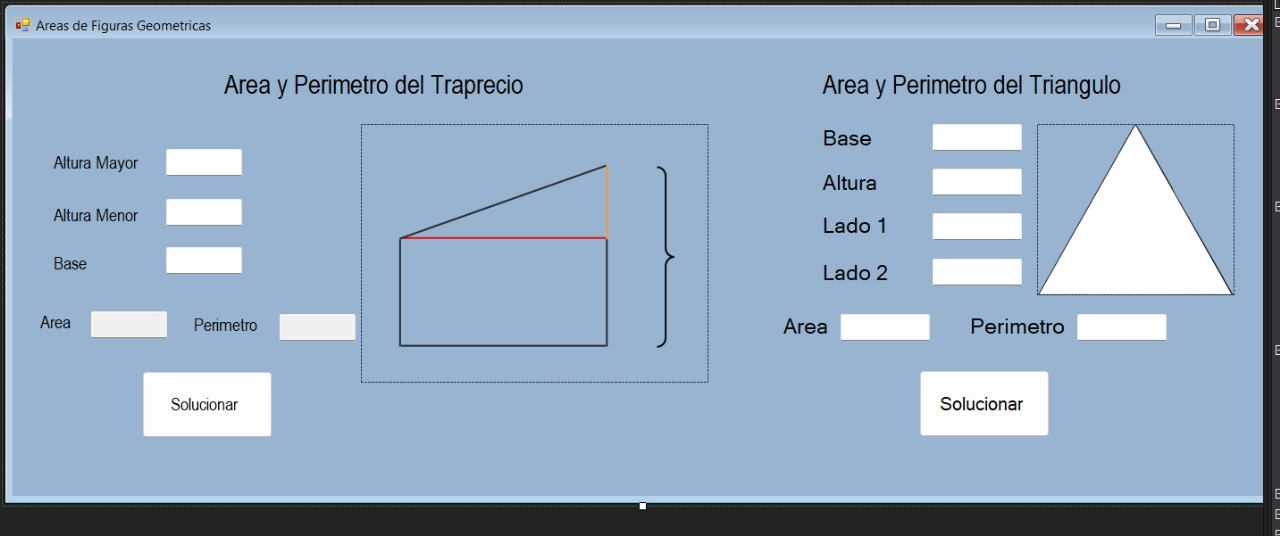
\includegraphics[scale = 0.5]{Imagenes/interfaz_grafica.jpeg}
  \caption{Interfaz Gráfica}{Fuente: Propia}
\end{figure}

\begin{figure}[H]
  \centering
  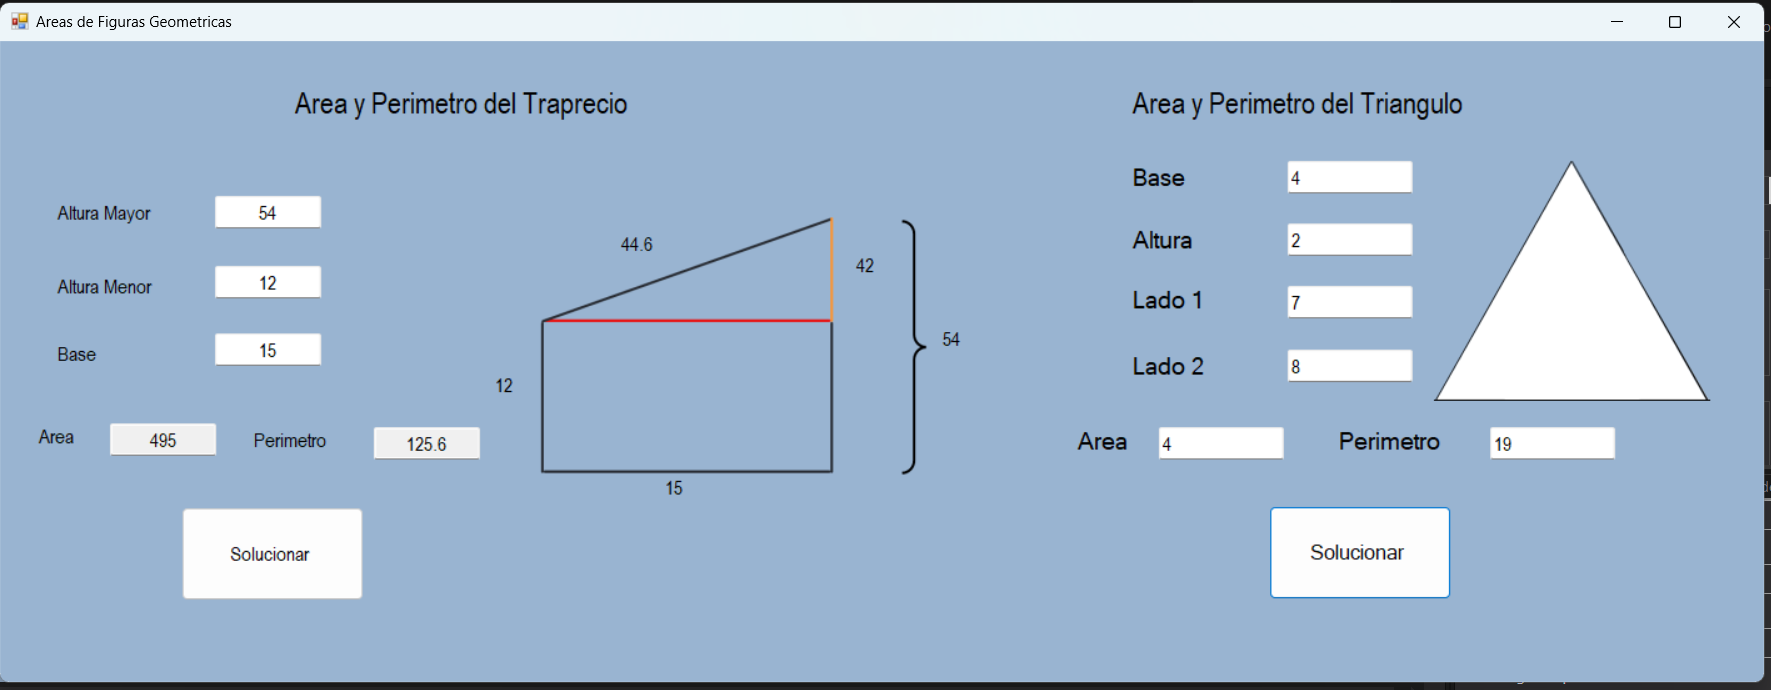
\includegraphics[scale = 0.5]{Imagenes/i2.png}
  \caption{Interfaz Gráfica}{Fuente: Propia}
\end{figure}


\begin{figure}[H]
  \centering
  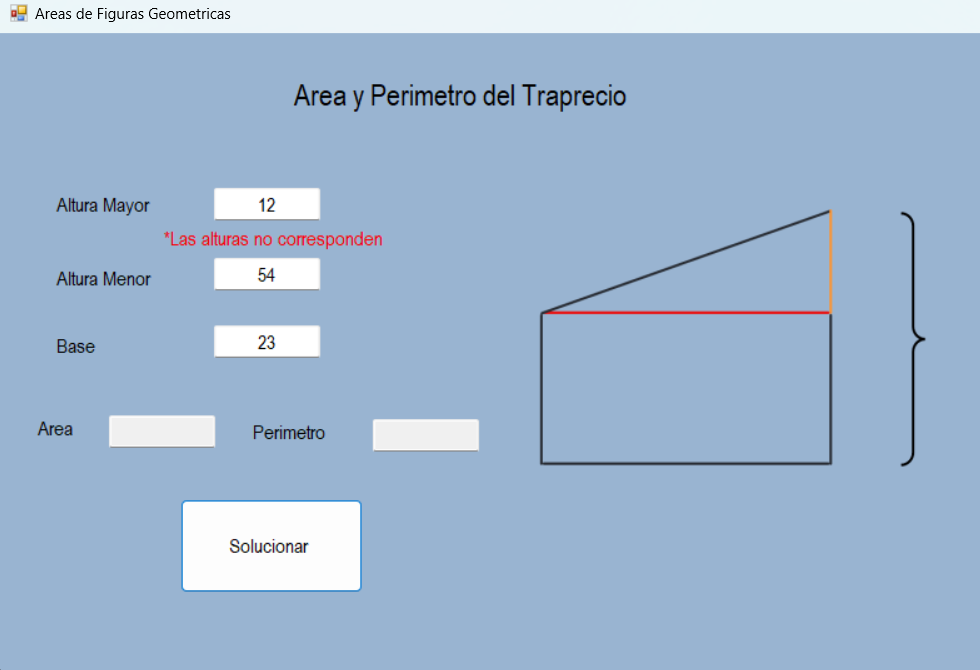
\includegraphics[scale = 0.75]{Imagenes/i3.png}
  \caption{Control de error}{Fuente: Propia}
\end{figure}
\chapter{Conclusiones}
A través de la realización de este programa, se logró implementar con éxito las fórmulas matemáticas para el cálculo del área y el perímetro del trapecio y el triángulo. La interfaz gráfica del programa permitió una interacción sencilla con el usuario, mejorando la experiencia de uso mediante una clara disposición de los campos de entrada y la visualización de resultados.

Además, el proyecto reforzó la importancia de validar los datos de entrada. Por ejemplo, se implementaron controles para asegurar que la altura mayor del trapecio fuera siempre superior a la menor, evitando así resultados incorrectos. Este ejercicio permitió aplicar tanto principios de geometría como habilidades de programación esenciales para el desarrollo de software práctico.
\chapter{Consideraciones Finales}
Este tipo de ejercicios proporciona una base sólida para la comprensión y aplicación de algoritmos matemáticos dentro de un contexto de programación. A medida que se avanza en la carrera de Ingeniería en Sistemas, la habilidad para traducir conceptos teóricos en soluciones automatizadas mediante el uso de herramientas de programación se vuelve cada vez más relevante.

Es importante señalar que, en futuros desarrollos, se podrían añadir más figuras geométricas para ampliar la funcionalidad del programa. Asimismo, la interfaz podría mejorarse mediante el uso de gráficos para representar las figuras geométricas basadas en los datos ingresados por el usuario, haciendo la herramienta más interactiva y visual.
\end{document}